\chapter{Résumé de thèse}
\label{chapter:IntroductionFR}

\section{Introduction}

Les progrès récents sur les modalités d'imagerie et de calcul numériques
ont ouvert un nouveau domaine d'étude de la variabilité biologique de l'anatomie humaine.
Ce nouveau domaine est appelé l' \textit{anatomie computationnelle} (CA).

La CA, telle que définie par \cite{Grenander1998}, possède trois aspects principaux : construction de
formes anatomiques ou modélisation par des points, des courbes, des surfaces et des volumes ;
Comparaison de ces modèles ; et l'analyse statistique de la variabilité de forme.

Les statistiques permettent de déduire et de tester des hypothèses d'états pathologiques.
Cela se fait à l'aide de tests statistiques qui déterminent la probabilité qu'une hypothèse soit vraie ou fausse.
Par exemple, un nouvel échantillon pourra être classé comme malade ou sain selon son score.

La construction automatique des modèles anatomiques
a été le principal intérêt de nombreux groupes de recherche dans le monde entier.
Ces modèles sont basés sur des algorithmes et des équations qui capturent le comportement
et/ou l'apparence de l'objet.

En plus des tests d'hypothèse, ces modèles sont également utilisés dans
différents types de procédures de simulation, par exemple, la simulation d'images médicales.
L'imagerie médicale consiste à acquérir des détails de l'intérieur du corps humain en utilisant différentes techniques physiques ou modalités.
Parmi ces modalités on retrouve entre autre : l'IRM (imagerie par résonance magnétique), le scanner X, les ultrasons (échographie) 
et la TEP (tomographie par émission de positons).
Elles sont employées couramment en clinique pour diagnostiquer et planifier les traitements des patients avec l'information "vue" dans l'image.
Ces dispositifs d'imagerie peuvent être très coûteux, ils nécessitent un entretien régulier et ne peuvent être utilisés que par un personnel qualifié.
Dans ce contexte, la simulation d'image médicale est définie comme le processus de production d'une image de synthèse
d'une modalité spécifique à l'aide de la géométrie d'un objet virtuel.
L'objet virtuel en question pourrait être un organe ou un système d'organes.

L'un des objectifs de la simulation d'image est l'amélioration des dispositifs d'imagerie.
Cela peut se faire quand la simulation améliore la compréhension des phénomènes d'acquisition, 
ou lorsque la simulation permet d'étalonner un ensemble spécifique de paramètres pour produire un résultat souhaité.
Une fois une simulation réussie, l'expérience peut s'effectuer sur l'appareil réel.
Une autre utilisation des images simulées est l'évaluation de la performance des algorithmes de traitement d'image, dont la segmentation.
Avec une image simulée, les résultats d'une segmentation peuvent être comparés directement au modèle d'objets virtuels.

D'autres types de simulations sont faites pour mieux comprendre les différents processus biologiques comme :
la déformation du muscle, le cycle cardiaque, le cycle respiratoire, le pliage corticale etc.

Sachant toutes les applications possibles dans le domaine médical,
le défi d'aujourd'hui est de créer un être humain virtuel.
Pour ce faire, il faut un modèle capable d'intégrer les informations anatomique, physiologique, mécanique,
biologique et physique.
Cet homme virtuel pourrait servir à améliorer les procédures de simulation
et aussi les tests d'hypothèse pour les états pathologiques.

Le premier objectif de cette thèse
est de fournir une technique assez 
générique capable de représenter la forme de divers organes.
Cette technique doit être capable d'inclure l'information
à différentes échelles spatiales.
Il existe de nombreuses approches permettant de modéliser la forme d'un objet.
Citons les modèles déformables, qui sont très utilisés dans ce dessein.
Ils sont notamment en mesure d'automatiser, dans une certaine mesure,
la segmentation de structures sur une image, et ils sont capables de produire des statistiques selon les déformations.
Malheureusement, ces techniques
ne permettent pas intrinsèquement leur utilisation dans un contexte de simulation réaliste d'organe.

Ce résumé de thèse est organisé de la façon suivante. 
La partie \ref{sec:3DModelsfr} résume les caractéristiques les
plus importantes de la méthode utilisée tout au long de cette thèse 
pour la modélisation de forme. Cette technique est appelée s-rep. 

La partie \ref{sec:cortexModelingfr} présente la contribution la
plus importante de ce travail de thèse.
Il s'agit d'une méthodologie permettant de créer une représentation de cortex.
Le modèle s'inspire du fait que la forme réelle du cortex est proche de celle d'une ``crêpe'' pliée.
Notons que la plupart des méthodes n'utilisent que l'information de surface.

Le deuxième objectif de notre représentation
est d'offrir un mécanisme
pour synthétiser des solides, c'est à dire les 
propriétés de la surface et les propriétés internes
de l'objet.
La procédure de synthèse utilise des échantillons de petites dimensions extraits d'images de référence.
Le résultat synthétisé est visuellement et statistiquement similaire à l'image de référence.
Les images texturées peuvent être de différentes sources comme
les images naturelles du web, l'histologie, ou plus complexes tel que des 
paramètres physiques.
Les solides générés peuvent être utilisés
pour améliorer la visualisation et/ou les propriétés internes des modèles créés
à l'aide de la technique décrite dans la partie \ref{sec:3DModelsfr}.
Le chapitre \ref{chapter:textureSynthesisfr} résume la procédure pour synthétiser les solides.

%Le troisième objectif est d'utiliser la description géométrique couplée avec les propriétés des paramètres physiques et générer des images simulées d'IRM.

Le troisième objectif est d'utiliser
la description géométrique couplée 
avec les propriétés des paramètres physiques
et simuler des images IRM.
Ces images sont validés avec des algorithmes de segmentation utilisés couramment.

La partie \ref{chapter:Conclusions} conclut ce résumé et annonce quelques perspectives à suivre.

\section{Représentation des objets en 3D}
\label{sec:3DModelsfr}
Les progrès technologiques ont permis 
le développement de modèles 3D de haute qualité. Ces modèles sont utilisés 
dans divers secteurs de l'industrie.
Ils décrivent l'apparence de l'objet d'une façon mathématique
et ils peuvent être utilisés dans l'animation, le prototypage et la simulation.
La géométrie de l'objet est au cœur de ces procédures.

Aujourd'hui, le défi est de créer des modèles d'objets adaptés
pour les procédures de simulations réalistes.
Ils doivent fournir les mécanismes permettant d'inclure les 
informations de diverses sources, à différentes échelles spatiales et 
permettant également de travailler avec plusieurs objets.
En plus, leur forme doit être représentatif d'une population.
Cela implique la mise en place d'une méthodologie pour calculer 
la moyenne des formes et une description de la variabilité dans une population.
Actuellement, il n'y a aucun formalisme bien établi
pour manipuler la forme, ni pour calculer une forme moyenne.
%Ceux sont plutôt difficiles tâches en vision par ordinateur.
% De façon généralisée, il devrait y avoir plus d'efforts pour comprendre
% Comment les mécanismes de la perception humaine
% traitent de forme comme ils le font très bien, mais ils ne sont pas complètement compris.

Élaborer un modèle avec les caractéristiques mentionnées ci-dessus,
ouvre la possibilité d'améliorer les procédures existantes de simulation;
d'acquérir une meilleure compréhension des systèmes du corps humain;
d'améliorer l'analyse automatisée sur les images médicales et
également d'améliorer la médecine personnalisée.
Les interventions médicales (non invasives) pourraient être planifiées à l'aide
des modèles ``patient spécifique'' s'ils ont été créés à partir
d'information acquise sur des images médicales.

La modélisation 3D se divisent en deux catégories : modélisation de surfaces et modélisation de solides (volumique).

Les modèles de surface représentent la couche externe de l'objet uniquement. 
Ils sont stockés comme un ensemble de primitives tels que des points, des arêtes ou des polygones qui définissent la frontière de l'objet.
Au cours des 20 dernières années, la plupart des recherches en représentation ont été faites sur cette catégorie car  plus facile à manipuler.
La modélisation des surfaces peut être divisée en deux sous-catégories : représentations de points saillants et
représentations de frontières ou b-reps.

En revanche, les modèles solides représentent l'extérieur et l'intérieur de l'objet.
Ils se divisent principalement en deux sous-catégories: les modèles basés sur la déformation d'un atlas et les représentations médian.
% Malheureusement, des modèles solides nécessitent plus de puissance informatique et ont été utilisés principalement à des fins de recherche.

Cette section fait un résumé des représentations médian
car c'est la technique utilisée pour les développements de cette thèse. 
Cette approche offre aussi des avantages pour décrire l'intérieur d'un objet, 
ce qui n'est pas le cas de nombreuses autres méthodes.
Le chapitre \ref{chapter:3DModels} donne une revue complète des techniques de représentations.

\subsection{Représentations médian}
\label{sec:quasiMedialfr}

\begin{chapquote}{Harry Blum}
  Pour une notion si simple comme l'emplacement d'un objet, la description par son contour ou périmètre est particulièrement pauvre.
\end{chapquote}

Le concept de représentation médian a commencé avec \cite{blum1967transformation}.
Blum a remarqué que pour toute forme, il était possible de calculer son axe médian. 
En le faisant, les objets pouvaient être décrits depuis l'intérieur vers l'extérieur, contrairement 
aux techniques qui cherchent à modéliser l'extérieur de l'objet uniquement.

Pour expliquer ce concept Blum a utilisé une analogie de ``champ en feu'', où la formation de l'axe médian se fait en mettant le feu à
la couche externe de l'objet. Le feu se propage uniformément vers l'intérieur de l'objet et
lorsque les fronts se rencontrent, nous trouvons l'axe médian.%, une notion liée aux courbes de niveau.
Suite à ce concept, la définition d'un axe médian est:

\begin{definition}
L'axe \textbf{médian} est la collection de points intérieurs équidistants avec au moins deux points sur la frontière de l'objet.
\label{def:medialAxis}
\end{definition}

Parallèlement au MA (axe médian) une MAT (transformation de l'axe médian) est générée:

\begin{definition}
La \textbf{transformation d'axe médian} est la distance de chaque point de l'axe médian à la frontière la plus proche de l'objet.
\end{definition}

Dans le contexte de l'analogie ``champ en feu'', la MAT ajoute à chaque point de l'axe une valeur équivalente à la durée de combustion depuis la frontière
jusqu'à ce que les deux fronts se rencontrent dans le MA.
La MAT a été critiquée vu que des petites perturbations sur la frontière produisent des changements significatifs
sur le MA, ce qui ne rend pas une description pratique de la forme d'un objet.
Cette instabilité a fait l'objet de nombreuses recherches qui visaient à produire un meilleur calcul du MA.
L'idée est d'identifier les sous-ensembles
significatifs qui composent le MA en échangeant l'exactitude contre la stabilité.

En général, pour accroitre la stabilité, un élagage du MA est fait par un seuil et un critère qui détermine
la ``substance'' et la ``connexion''. La substance étant la partie concrète de l'objet, et la connexion, comment les pièces sont reliées.
Pour avoir une meilleure compréhension de cette notion on peut imaginer une main.
Une main est composée par une paume (un bloc) et des doigts (des protubérances) ou
considérez-la comme une collection d'objets connexes. 
La substance est connectée d'une telle manière que nous percevons un main.
L'objectif est donc de trouver ces connexions.

Différents auteurs proposent des approches pour calculer un MA stable : voir les méthodes de
\cite{culver1999accurate}, \cite{amenta2001power}, \cite{katz2003untangling}, \cite{miklos2010discrete}.

Un MA stable est un descripteur de forme puissant qui
produit représentations compactes de la forme et de la surface d'un objet.
Les concepts ``point central'' et positions à l'intérieur et par rapport à l'objet
sont decrits plus efficacement à l'aide du MA.

En 2D, le MA est créé à partir des centres des cercles de rayon maximal ayant au moins deux
points en commun avec la frontière de l'objet. L'union des centres de ces cercles forme le MA.
En 3D le MA est composé des feuilles générées avec les centres des sphères de rayon maximum inscrites dans l'objet.
De manière générale, le MA s'étend dans les dimensions supérieures, où il est défini à partir d'hypersurfaces
générées avec les hypersphères de rayon maximum inscrites dans l'objet.

Une question importante liées aux représentations médian
est de savoir si les analyses statistiques sont viables sur une population d'objets.
La principal difficulté consistera à produire la correspondance des structures.
Pour utiliser une représentation médiale pour l'analyse statistique de la forme,
la construction du MA s'effectuera d'une manière différente:
le MA doit avoir une structure stable pour la population d'objets que nous voulons étudier.

Si nous prenons en considération comment le MA est construite, 
nous voyons que la procédure est une approche haut-bas,
Elle commence à la frontière de l'objet et en utilisant la procédure pour inscrire des sphères, le MA est obtenu.
La deuxième alternative consiste à construire le MA dans le sens inverse.
\cite{styner2001medial} propose une approche bas-haut pour construire le MA.

Pour résumer, la méthode de Styner calcule un MA moyen
d'une population d'objets suivi d'un échantillonnage de la moyenne 
en utilisant une grille régulière des points. 
La grille de points est ajustée à la moyenne. Le résultat est utilisé comme le nouveau MA.

Pour calculer la moyenne du MA, une PDM (modèle de distribution de points) 
est créée à partir des représentations en SPHARM (harmoniques sphériques)
des MA calculés pour chaque objet dans la population.
Une PCA (analyse des composantes principales, voir Annexe \ref{sec:apendixPCA})
est faite sur la PDM. Cette analyse permet de calculer une moyenne, dans ce cas un MA moyen.
Enfin, la grille de points ou m-rep (définition donnée ci-après) 
est ajustée à la moyenne par la minimisation d'une fonction de distance sur les points.
Une série de tests est exécutée pour évaluer si le m-rep 
représente correctement chaque objet, ainsi que la population en général.

Un m-rep est un objet continu qui définit le MA d'un objet comme
un ensemble d'espaces topologiques \cite{pizer1999segmentation}, \cite{yushkevich2003continuous}, \cite{pizer2003deformable}.
La MS (feuille médiale en 3D, équivalent à MA en 2D)
est paramétrée par $MS (u, v)$ où $u$ et $v$ peuvent prendre toutes valeurs comprises entre $[0, 1] \in R$.
La MS est un ensemble continu $C^2$ d'atomes médiales avec 
une surface implicite $y_{0}$ pour la surface supérieure et $y_{1}$ pour la surface inférieure.

\begin{equation}
MS (u, v) = \{x, r, n_0, n_1\}
\label{equ:medialSheetAtomFR}
\end{equation}

L'équation \ref{equ:medialSheetAtomFR} définit un atome pour chaque $(u, v)$ sur la MS,
$x$ correspond à la position sur la MS, $n_0$ et $n_1$
sont des vecteurs et $r$ est la longueur de ces deux vecteurs (n_0 et n_1 sont des vecteurs normalisés).


Un autre type d'atome se trouve sur les bords de l'objet, nommé atome de crête.
La crête est chargée de joindre les surfaces supérieure et inférieure
pour produire un contour fermé.

Pour décrire un m-rep informatiquement,
un ensemble discret d'atomes est utilisé.
Par la suite, le mot m-rep fait référence à la version discrète de l'objet.
Les m-reps utilisent les mécanismes d'interpolation décrits dans \cite{thall2004deformable},
pour reconstruire la surface de l'objet.
La surface interpolée est en correspondance
aux normales décrites par les vecteurs $n_0$ et $n_1$.
La surface est $C^2$ continue partout.
% De méthode de ce Thall surface permet de calculer les atomes médianes interpolées.

En résumé, les m-reps sont des structures 
qui décrivent efficacement la géométrie d'un objet d'une manière multi-échelle.
Ils peuvent être utilisés pour la segmentation des images médicales \cite{pizer2005method} 
et pour effectuer
des analyses statistiques sur la variabilité de forme \cite{fletcher2004principal}.
La méthode employée par m-reps pour produire des statistiques est appelée PGA (analyse des géodésiques principales)
une généralisation de la PCA (analyse en composantes principales).

La PGA décrit les variations sur les espaces sphériques avec des grands cercles.
Malheureusement, les données d'un m-rep vit fréquemment sur petits cercles
et la description de la variabilité avec une PGA n'est pas optimale.
Un méthode plus appropriée peut être développée en prenant en compte cette information.

La section suivante fait un résumé des s-reps, la technique développée et utilisée tout au long de cette thèse.

\subsection{Représentations quasi-médian}

Les représentations quasi-médian \cite{pizer_nested_2012} ou s-reps, 
diffère des représentations médian dans le critère strictement médial imposée sur chaque atome. 
C'est-à-dire, la position d'un atome n'est pas nécessairement le centre
d'une sphère inscrite au maximum.
Dans un s-rep, les atomes sont récompensés pour être dans le centre de la sphère mais des petits
écarts sont tolérés, ce qui signifie que les rayons (vecteurs vers la surface) peuvent avoir différentes longueurs;
Cela se fait dans l'objectif d'améliorer l'ajustement du s-rep à un objet donné.

Les s-reps sont des objets continues, définies comme un locus (lieu central) de vecteurs $(p, S)$
avec la queue situé à $p$ et une direction qui pointe vers $p + S$. 
Également, ils sont paramétrés par $(u, v)$ tels que
la feuille squelettique est définie comme $SS = \{p (u, v): \in \forall (u, v) [0, 1] \} $, les
vecteurs $SP = \{S (u, v): \in \forall (u, v) [0, 1] \} $ et
la frontière de l'objet est $BO = \{p (u, v) + S (u, v): \in \forall (u, v) [0, 1] \} $.
L'union des queues forme le locus squelettique comme un 
un feuille entièrement plié, c'est-à-dire, la partie supérieure de la feuille est paramétrée par $v \in [0, 0.5] $
et la face inférieure par $v \in [0,5; 1]$.
Selon cette définition, tous les points à l'intérieur de l'objet sont accessibles par au moins un vecteur;
il faut faire attention aux coins de l'objet car ils sont atteints par plusieurs vecteurs mais ils permettent 
à la SS de se plier et créer cette représentation d'objet avec une description interne.

Les longueurs des vecteurs sont définis comme $r (u, v) = |S (u, v) | $ et
les directions des rayons comme $U (u, v) = S (u, v) / r (u, v) $.

La Section \ref{sec:internalCoordinates} explique en détaille les notions sur la description interne d'un objet
et la génération des cartes $X2U$, qui permettent le passage d'une coordonnée physique à une coordonnées s-rep.
Ces cartes seront utilisées dans le Chapitre \ref{Chapter:MRISimulation} pour augmenter 
les propriétés des s-reps avec information volumétrique.

%\begin{figure}
%\centering
%\subfigure[slabular]{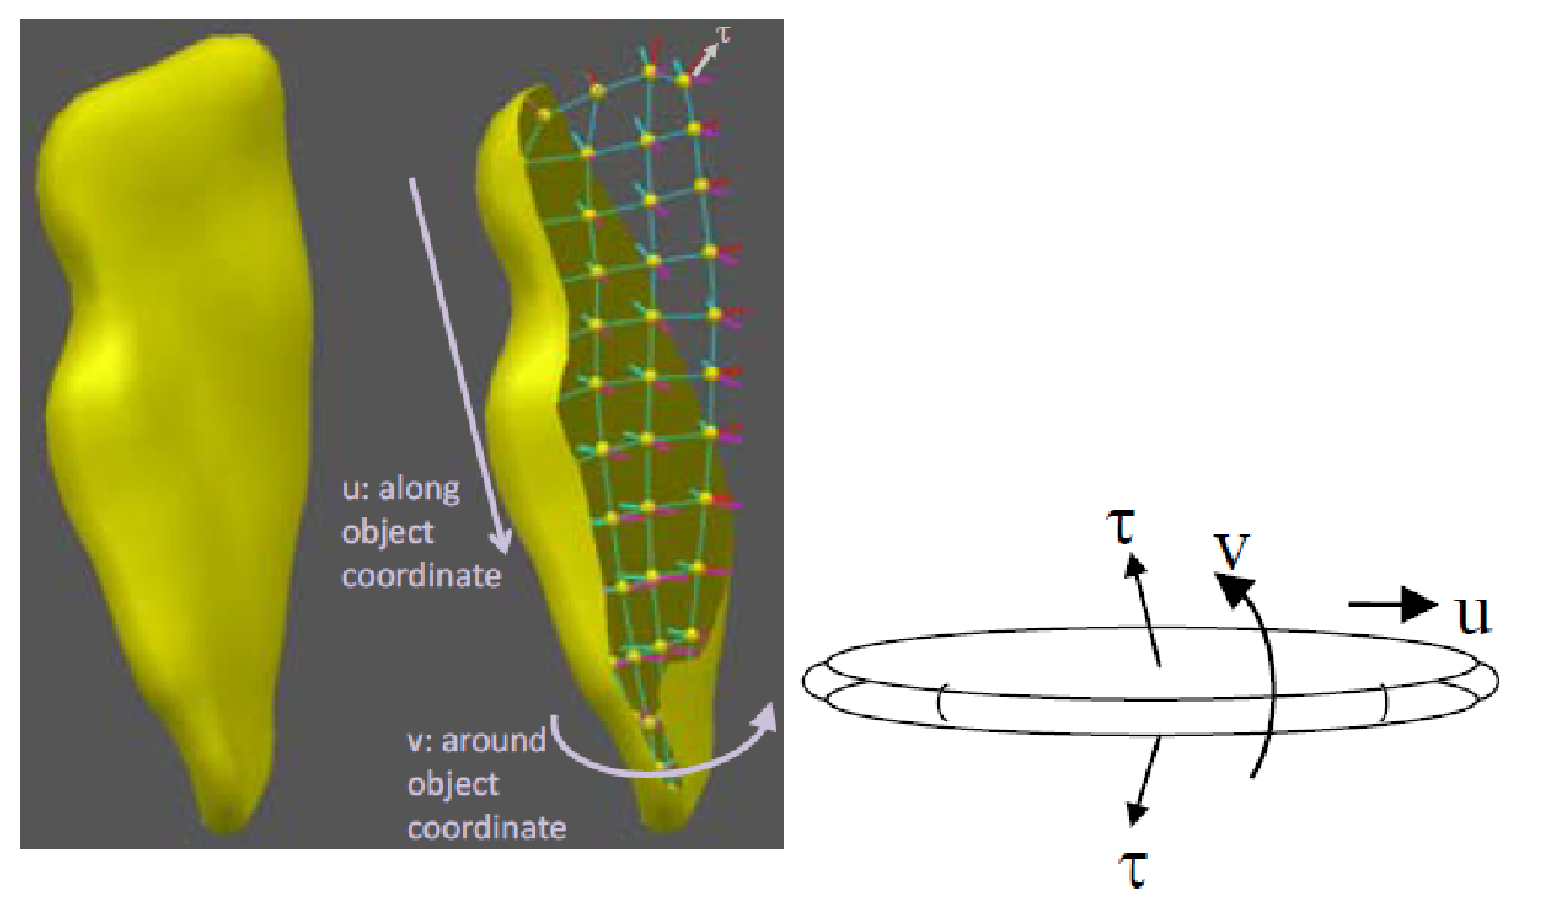
\epsfig{file = s-repSlab.eps, width = 16 cm}}
%\subfigure[quasi-tube]{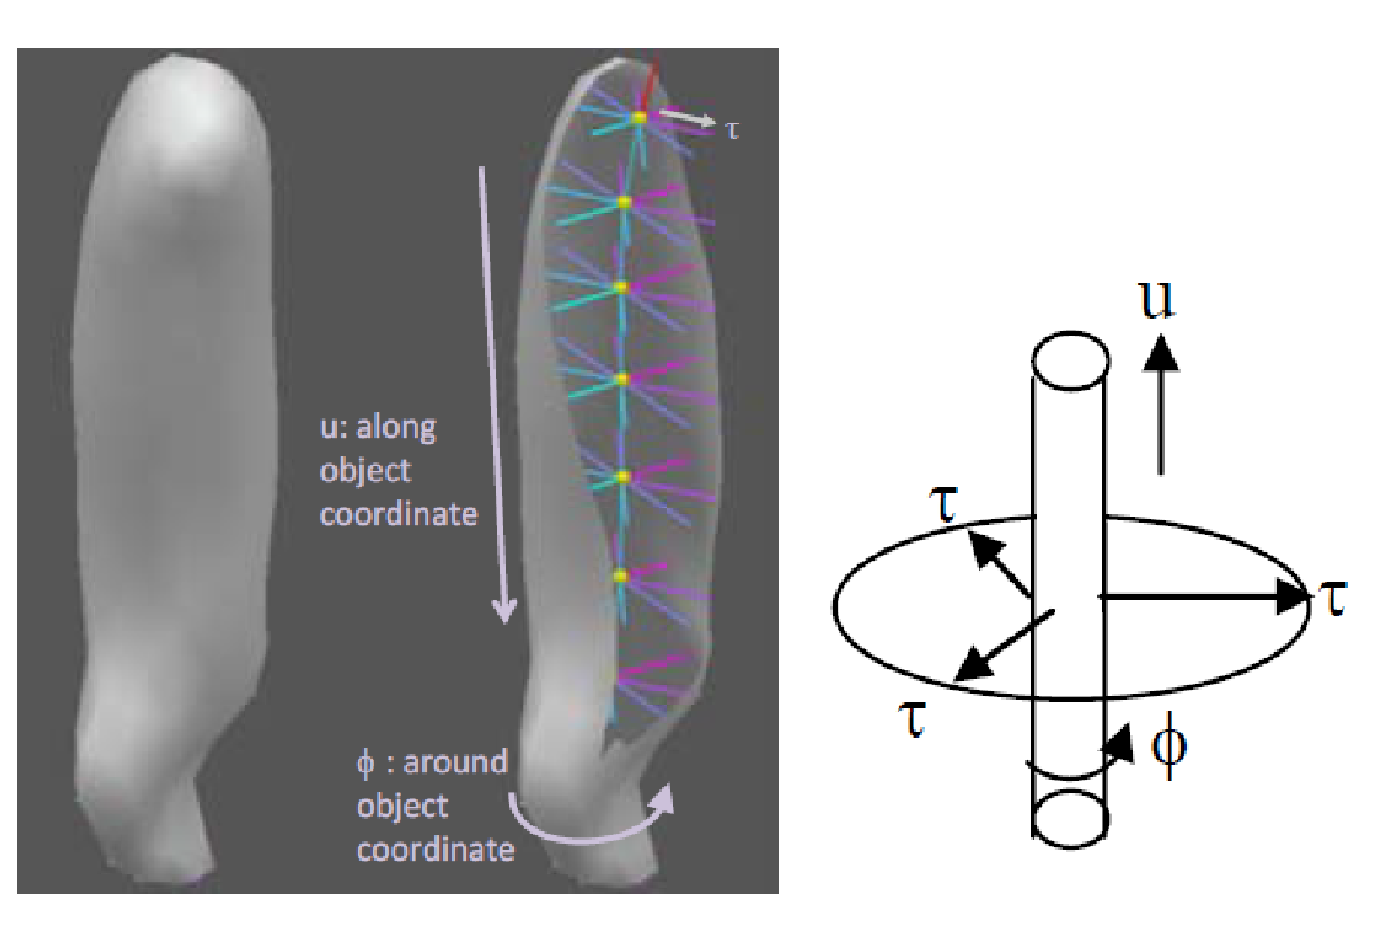
\epsfig{file = s-repTube.eps, width = 16 cm}}
%\caption[SLAB de type s-rep.]{Image extraite de \cite{pizer_nested_2012}. Dalle S-rep, intérieur, objet de remplissage. Paramétré par \in [0, 1] $ (u, v, \tau)$
%chaque point à l'intérieur de l'objet sont accessibles par un seul a parlé.
%De même, une figure de tube est paramétrisée par $(u, \phi, \tau)$, $\phi$ est la rotation autour de la courbe de l'espace qui définit la MA.}
%\label{Fig:srepFigure}
%\end{figure}

D'une façon similaire aux m-reps, les s-reps sont représentés avec un ensemble discret d'atomes.
Par la suite, s-rep fait référence à la version discrète de l'objet.
Les s-reps utilisent les mécanismes d'interpolation décrits dans \cite{damon2003smoothness},
\cite{han2006interpolation}, \cite{damon2008swept}. 
Avec ces mécanismes d'interpolation, la surface de l'objet ainsi que 
tout les positions internes de l'objet peuvent être trouvés.

En plus de la modélisation de forme en utilisant les mécanismes d'interpolation,
le but est de produire des s-reps utilisables pour des analyses statistiques.
Pour calculer des statistiques sur un ensemble d'objets, la SS d'un s-rep doit rester
stable dans chaque instance de la population d'objets.

Les résultats statistiques sont robustes quand les points saillants des objets
sont en correspondance dans la population.

Tout d'abord, un s-rep est créé à partir d'un image binaire.
Cela est obtenu 
par des méthodes de segmentation automatique ou manuel (contours)
aux images médicales d'un certaine modalité.

Avec cette image binaire, une transformé de distance est calculé. La transformé de distance 
associe un valeur de distance à chaque point de l'image au point plus proche de la frontière 
de l'objet. Les points à l'intérieur de l'objet ont des valeurs négatifs, les points
à l'extérieur de l'objet ont des valeurs positifs, et les points dans la frontière sont égale à 0.

Un procès d'ajustement est utilisé
pour aligner le s-rep à l'image binaire. 
Ce procès est guidée par le calcul des gradients dans la transformé de distance.
L'ajustement a principalement 3 étapes:
la première étape consiste à aligner le s-rep sur l'image ;
la deuxièmement étape consiste à déplacer chaque atome séparément (le mouvement d'un atome modifie la surface) ;
la troisième étape consiste a modifier les longueurs des vecteurs vers la surface.

Avec cette procédure, une figure squelettique de base peut être placé sur 
un ensemble d'images binaires. Le procès d'ajustement crée la meilleure représentation
pour l'image binaire et augmente la correspondance des positions d'objet à travers la population.

L'ensemble de s-reps contiennent une squelette stable et modélisent les objets dans la population, 
CPNS (composite principal nested spheres voir Annexe \ref{sec:apendixCPNS}) est utilisé pour le calcul
de statistiques de forme.

CPNS produit une forme moyenne et un ensemble de modes propres.
Tous les formes dans la population peuvent être modéliser
avec un ensemble de coefficients la forme moyenne et les modes propres.
En général, il est possible de calculer statistiques robustes pour la forme d'objets 
en 3D à l'aide des représentations médiales.
 
La section suivante fait un résumé pour expliquer 
la mise en œuvre de représentations médiales.

\subsection{Modélisation d'objet avec s-reps}
\label{sec:s-repImplementationfr}

\subsubsection{Interpolation de la feuille médian}

L'interpolation de la feuille médian est faite avec splines cubiques d'Hermite.
Pour produire l'interpolation, les dérivées partielles pour chaque atome sur la SS,
et la normale doivent être définie.

Sois $s_{rep} = \{(p_i, S_i) : i \in N\}$ et $N = m \times n$, 
un s-rep est représenté par une grille discrète d'atomes.
L'interpolation utilise les quatre points de contrôle dans chaque quadrangle de la grille.

%A quad est défini comme
% $MMO {i, j} = \{S (i/n, j/m), S ((i+1)/n, j/m), S ((i+1)/n, (j + 1) /n), S (i/n, (j + 1) / m): J'ai \in [1, n], \in j [1 m] \}] $)),
Les équations \ref{equ:pDerivativeUFr} et \ref{equ:pDerivativeVFr} indique comment calculer la dérivée partielle pour un atome 
dans le sens de $u$ et de $v$ sur la SS. $\Delta u = 1/m$ et $\Delta v = 1/n$
correspond à la longueur de déplacement. $u + \Delta u$ se déplace le long de la direction $u$ au
prochain atome sur la grille des atomes discrètes, de la même façon pour la direction $v$.

\begin{equation}
 \partial p(u, v)_u = \left \{ \begin{array}{ll}
                      p(u + \Delta u, v) - p(u , v) & u = 0\\
                      \big (p(u + \Delta u, v) - p(u - \Delta u, v)\big )/2 & 0 < u < 1 \\
                      p(u, v) - p(u - \Delta u, v) & u = 1
                     \end{array} \right .
\label{equ:pDerivativeUFr}
\end{equation}

\begin{equation}
 \partial p(u, v)_v = \left \{ \begin{array}{ll}
                      p(u, v + \Delta v) - p(u, v) & v = 0\\
                      \big (p(u, v + \Delta v) - p(u, v - \Delta v) \big ) /2 & 0 < v < 1 \\
                      p(u, v) - p(u, v - \Delta v) & v = 1
                     \end{array} \right .
\label{equ:pDerivativeVFr}
\end{equation}

L'équation \ref{equ:sheetNormalFr} donne une approximation à la normale d'un atome à la SS.
La normale est calculée à partir des vecteurs situés à la même position sur la SS
mais directions opposées.

\begin{equation}
  \begin{array}{cc}
   N(u, v) \approx \frac{S(u, v) - S(u, 1 - v)}{||S(u, v) - S(u, 1 - v)||}  & u  \in [0, 1], v \in [0, 0.5] \\
  \end{array}
\label{equ:sheetNormalFr}
\end{equation}

\begin{equation}
 H_{control} = \left [ \begin{array}{cccc}
                    p_{11} & p_{12} 			& \partial p_{{11}_v}^T & \partial p_{{12}_v}^T \\
                    p_{21} & p_{22}			& \partial p_{{21}_v}^T & \partial p_{{22}_v}^T \\
                    \partial p_{{11}_u}^T & \partial p_{{12}_u}^T	& h_{0} & h_{0} \\
                    \partial p_{{21}_u}^T & \partial p_{{22}_u}^T	& h_{0} & h_{0} \\
                    
                   \end{array} \right ]
  \label{equ:hermiteControlFr}
\end{equation}

Pour interpoler la SS, un matrice d'Hermite est défini dans l'équation \ref{equ:hermiteControlFr},
où $\partial p(u,v)^T = \partial p(u,v) - (\partial p(u,v) \cdot N(u, v))N(u,v)$ est la projection 
des dérivés discrets dans les directions $u$ où $v$ sur les plans de la tangente
qui sont déterminés par les normales $N(u,v)$. 
L'interpolation de la SS dépend des normales et des dérivés discrets; $h_{0}$ est un vecteur rempli de $0$.

\begin{equation}
 \begin{array}{l}
  H_1(s)= 2s^3 - 3s^2 + 1\\
  H_2(s)= -2s^3 + 3s^2\\
  H_3(s)= s^3 - 2s^2 + s\\
  H_4(s)= s^3 - s^2\\
 \end{array}
\label{equ:weightFunctionsFr}
\end{equation}

\begin{equation}
 p(u, v) = \left [ \begin{array}{cccc} H_1(\hat u) & H_2(\hat u) & H_3(\hat u) & H_4(\hat u) \end{array} \right ]
                H_{control}
           \left [ \begin{array}{c} H_1(\hat v) \\
				     H_2(\hat v) \\ 
				     H_3(\hat v) \\ 
				     H_4(\hat v) 
		    \end{array} \right ]
\label{equ:interpolatedPointFr}
\end{equation}

La position interpolée d'un atome quelconque sur la SS est indiquée dans l'Équation \ref{equ:interpolatedPointFr},
en utilisant un patch de control de matrice de Hermite et les fonctions de poids définies dans l'Équation \ref{equ:weightFunctionsFr}.
$\hat u = (u - floor(u)) / \Delta u$, où $floor(u)$ retourne la coordonnée $u$ de l'atome à $p_{11}$,
de même pour $\hat v$.

De manière similaire, l'interpolation des vecteurs peut être faite à l'aide de fonctions d'Hermite. Au lieu d'utiliser les points de contrôle
$p (u, v)$, les vecteurs $S (u, v)$ sont utilisés. En conséquence, les dérivés discrets sont calculés pour chaque vecteur, la différence
dans ce cas est qu'aucune projection est fait en utilisant les normales à la SS ; l'interpolation des vecteurs ne dépend que des dérivés discrets.

La surface supérieure et inférieure peut être générée à l'aide des mécanismes décrits ci-dessus.
La surface supérieur et inférieur se rencontrent à la crête de l'objet.
La section suivant explique comment effectuer l'interpolation de la crête pour produire la surface complet de l'objet.

\subsubsection{Interpolation de crête}
\label{sec:crestInterpolationfr}

Pour interpoler la crête, nous voulons créer une surface qui
ne s'effondre pas vers l'intérieur de l'objet, \textit{i.e.},
sa section doit être convexe dans la direction principale et préserver la continuité $C^2$. 
La surface doit aussi correspondre aux dérivés partielles afin de produire une surface lisse.

La méthode d'interpolation de crête est expliquée en montrant comment interpoler les longueurs $r$ 
entre deux vecteurs selon un angle $\theta$.
La fonction $r(\theta)$ renvoie la longueur à un angle donné.
De façon similaire, nous voulons interpoler la section transversale de la crête, où thêta
paramètre le parcoure du vecteur qui point vers la surface supérieur jusqu'au vecteur qui point 
vers la surface inférieur.

La même problématique peut être étendu à trois dimensions où l'interpolation produit une courbe d'espace.
Afin de produire une surface interpolée, la section section transversale
balaie le long de la crête ou le bord de la SS.

\begin{equation} 
 \frac{\partial^2 r(\theta)}{\partial \theta} = q_0  +  q_1  \theta + q_2  \theta^2  
 \label{equ:curvaturefr}
\end{equation}

La première étape consiste à définir une fonction quadratique de la courbure, comme montré dans l'équation
\ref{equ:Curvaturefr}, nous voulons avoir une courbe convexe interpolée.
En intégrant cette équation deux fois, nous trouvons la fonction qui donne la longueur pour $\theta \in [0, \theta_{max}]$.

\begin{eqnarray} 
  \frac{\partial r(\theta)}{\partial \theta} &=& \int_0^{\theta_{max}} \frac{\partial^2 r(\theta)}{\partial \theta} \partial \theta \\
  \frac{\partial r(\theta)}{\partial \theta} &=& \frac{\partial r_0}{\partial \theta} + q_0  \theta + \frac{1}{2}  q_1  \theta^2 + \frac{1}{3}  q_2  \theta^3  \\
  r(\theta) &=& \int_0^{\theta_{max}} \frac{\partial r(\theta)}{\partial \theta} \partial \theta \\
  r(\theta) &=& r_0 + \frac{\partial r_0}{\partial \theta}  \theta + \frac{1}{2}  q_0  \theta^2 + \frac{1}{6}  q_1  \theta^3 + \frac{1}{12}  q_2  \theta^4  
\end{eqnarray}

Nous allons commencer par résoudre les coefficients de $q_1$ et $q_2$,
en utilisant le système d'équations $r(\theta)$, $\partial r(\theta)/\partial \theta$ et $\partial^2 r(\theta)/\partial \theta$, 
comme indiqué dans l'équation \ref{equ:solveQ1fr}.

\begin{eqnarray} 
q_2 &=& \frac{6}{\theta_{max}^4} (2 \partial r_{end} \theta_{max} + q_0 \theta_{max}^2 - 6 r_{end} + 6 r_0 + 4 \partial r_0 \theta_{max}) \\
q_1 &=& \frac{-6}{\theta_{max}^3} (-\partial r_{end} + r_0 + \partial r_0 \theta_{max} +  \frac{q_0}{2} \theta_{max} + \frac{q_2}{12} \theta_{max}^4)
\label{equ:solveQ1fr}
\end{eqnarray} 

Il existe une solution au problème pour chaque $q_0$, mais
la solution optimale se trouve lorsque $q_0$ minimise 
tel qu'indiqué dans l'équation \ref{equ:minimizeCurvaturefr}.

\begin{equation}
 \partial r_{end} =  -1 \partial r_{end} = 0 \partial r_{end} = 1 r_0 \theta \partial r_0
\end{equation}

\begin{equation}  
  \hat q_0 = \operatorname*{arg\,min}_{q_0} \sum_{\theta = 0}^{\theta_{max}} \frac{\partial^2 r(\theta)}{\partial \theta}
  \label{equ:minimizeCurvaturefr}
\end{equation}

Pour produire un courbe d'espace, le méthode s'est fait séparément pour $[x, y, z]$.
En utilisant l'information discrète donnée par le s-rep,
il est possible de récupérer les positions $p_0$, $p_{fin}$ et calculer les dérivés discrets $\partial p_0$ et $\partial p_{fin} $
qui sont les paramètres nécessaires pour l'ajustement de la courbe.
Les atomes de crête du s-rep sont considérées comme un boucle
où les positions de crête sont données par $cp_n$ où $n$ est le nombre de positions de crête.
Les dérivées directionnelles sont calculées comme $\partial cp_j = (cp_{j + 1} - cp_{j - 1}) / 2$
qui sont projetés sur le plan tangent, donné par les normales de la SS à chaque atome
$\partial \hat {cp_j} = \partial cp_j - (\partial cp_j \cdot N_ {cp_j}) N_ {cp_j} $.

Le même mécanisme d'interpolation est utilisé pour les vecteurs en haut, crête et en bas,
par conséquence, pour un $t$ donnée,
il est possible de trouver le vecteur de haut $CS(t)^1$, le vecteur de crête $CS(t)^0$ et le vecteur de bas $CS(t)^{-1}$;
plus la position sur la crête de l'objet.

Enfin l'interpolation est fait pour cette ensemble de vecteurs, 
ce qui permet de produire la surface de crête interpolée de $haut \rightarrow bas$.

La section suivante faite un résumé sur les coordonnées internes d'un s-rep car 
ce mécanisme permet d'augmenter les propriétés internes des s-reps.

\subsubsection{Coordonnées internes d'un s-rep}
\label{sec:internalCoordinatesfr}

Les coordonnées internes d'un objet sont décrits par cartes $X2U$.
Ces cartes permettent la requête des coordonnées spatiales $[x, y, z]$
et retourne des coordonnées relative à l'objet $[u, v, \tau]$.
Les cartes $X2U$ serviront dans la Section \ref{sec:IRMSimulationfr}
pour mapper les solides générés avec la méthode décrit dans la Section \ref{sec:textureSynthesisfr}.
Cela est possible parce que les solides sont synthétisées
dans un cube. Chaque point dans le cube peut être liée à $[u, v, \tau]$, fournissant ainsi,
un mécanisme pour mapper un solide dans un s-rep.

Pour créer un carte $X2U$, 
chaque vecteur dans la SS (la feuille squelettique) du s-rep  est représenté par 
une coordonnée $[u, v]$.
$\tau$ est utilisée pour représenter la longueur du vecteur jusqu'à la surface.

Grâce aux mécanismes d'interpolation de la SS et des vecteurs (haut, bas et crête),
la fonction $U2X(u, v, \tau) = [x, y, z] | (u, v, \tau) \in [0, 1]) $ 
donne la position en coordonnées  physiques $[x, y, z]$ correspondant 
aux coordonnées $[u, v, \tau]$ de l'objet.
$v \in [0, 0.5] $ fait référence aux vecteurs dans la face supérieur
et $v \in [0,5; 1]$ fait référence aux vecteurs dans la face inférieure
du s-rep par rapport à la SS.

En utilisant la fonction $U2X$, la carte $X2U$ 
de l'objet est créée.
Avect un carte $X2U$, l'accés aux coordonnées d'objet est fait avec une complexité 
de $O(1)$.

\subsection{Conclusions}
\label{sec:3dRepConclusionfr}

Les s-reps sont capables de modéliser l'espace continue dans un objet.
Il y a la possibilité d'inclure 
de l'information de façon multi-échelle à la représentation géométrique.
Cette caractéristique est utilisé
pour inclure les paramètres nécessaires pour effectuer une simulation d'IRM.

En plus des possibilités de description interne d'un objet,
les s-reps sont adaptés pour le calcul de la variabilité statistique de forme 
sur une population d'objets modélisée avec la même SS.
Ce calcul de variabilité statistique est fait avec CPNS.
Par conséquence, tout les objets dans la population 
peuvent être décrits avec quelques coefficients, et la forme moyenne 
et les modes propres obtenus avec l'analyse via CPNS.

La section suivant explique une nouvelle méthodologie pour
modéliser le cortex du cerveau avec s-reps.
Avec cette structure une analyse statistique est menée à l'aide du CPNS,
ce qui prouve que les s-reps sont bien adaptées pour modéliser des
structures complexes.

\section{Modélisation du cortex via s-reps}
\label{sec:cortexModelingfr}

\subsection{Introduction}
\label{sec:introductionfr}

Le cortex cérébral à la forme d'une feuille pliée de tissu neuronal
avec d'interconnexions compactes qui permettent le traitement d'information.
Il joue un rôle important dans la mémoire, l'attention, la perception, la pensée, le langage et la conscience.
Des avancements ont été réalisés pour comprendre la structure et la fonction du cortex.
\cite{lorente1934studies} a proposé que le cortex est formé par petites cylindres qui contient des chaînes verticales des neurones ;
Ces structures ont été appelées colonnes, et ils correspondent 
aux groupes de cellules perpendiculaires à la surface corticale.
Cette hypothèse a été confirmée avec les études physiologiques faites par \cite{mountcastle1998perceptual}.

Le cortex est une feuille stratifiée avec une structure cellulaire plus ou moins uniforme.
Aujourd'hui, l'organisation colomnaire est le modèle établie pour expliquer le traitement 
de l'information dans le cortex.

Presque deux tiers de la surface corticale est cachée dans les sillons, il est difficile d'effectuer des analyses statistiques et de la visualisation.
Différentes procédures ont été élaborées pour déplier et mapper la surface corticale sur différents espaces (gonflés, sphériques ou aplaties)
\cite{drury_computerized_1996}, \cite{hermosillo_unfolding_1999}, \cite{fischl_cortical_1999}, \cite{pons_area_2004}.
Cela permet à la surface corticale d'être analysée et visualisée. Des méthodes statistiques 
peuvent être appliqués sur ces espaces aussi.
\textit{Freesurfer} (un outil automatisé pour la reconstruction de la surface corticale du cerveau à l'aide des données d'IRM structurelles)
utilise le procedure de gonflement et d'aplatissement de \cite{fischl_cortical_1999}.

De la même façon, l'évolution du cortex a été un sujet de grand intérêt.
Une grande partie des efforts ont aidé à comprendre comment le procès de pliage se produit.
Les pliage sont uniques à chaque cerveau et un repliement anormal est liée aux
problèmes neurologiques comme la schizophrénie, l'épilepsie, l'autisme et le syndrome de Down.
Pour une revue récente sur les théories de pliage voir \cite{filas2013mechanisms}.

Il y a de possibilités de recherche dans le développement des modèles du cortex.
Comme indiqué par Javier de Felipe \cite{defelipe2012neocortical}, ''il est encore nécessaire
d'atteindre une meilleure compréhension fondamentale sur les colonnes corticales
et comment elles sont utilisées dans les processus du cortex. En conséquence, il
est important de traduire ces dernières avancées techniques et
découvertes en neurosciences en applications pratiques pour
les neuroscientifiques, les cliniciens et pour ceux qui s'intéressent à l'anatomie 
comparatif et évolutif du cerveau.''.

Compte tenu de ces faits, l'un des objectifs de cette thèse est de fournir un
outil qui modélise la forme du cortex et se rapporte à la structure physique réel.
La Section \ref{sec:s-repImplementationfr} définit un s-rep
avec les mécanismes d'interpolation correspondants pour paramétrer l'intérieur de l'objet en $[u, v, \tau]$.
Les s-reps peuvent être utilisés pour modéliser les informations anatomiques et physiologiques des différentes couches du cortex.
Cette information peut être incluse naturellement à l'aide de la coordonnée $\tau$.

En plus de fournir une description de forme, les s-reps ont été utilisés avec succès pour le calcul
statistique sur la forme et le calcul de la forme moyenne sur une population d'objets.
%, Cela se fait à l'aide du CPNS une méthode analogue à l'APC \cite{pizer_nested_2012}.
Avec cette description statistique, il semble possible de classifier des objets selon ça forme.
% La majorité n'utiliser les informations de surface ; en revanche, la structure du squelette apporte
% stabilité aux statistiques et augmente la correspondance de l'information dans l'ensemble de la population d'objets.
%S-reps ont été utilisés pour modéliser les structures du cerveau interne comme l'hippocampe \cite{pizer_nested_2012}.
Les objets modélisés avec s-reps jusqu'à présent sont simples. La plupart d'entre eux ont une
forme de type arrondi ou allongé comme celle de l'hippocampe \cite{pizer_nested_2012}.

Il est démontré que les s-reps sont capables de représenter une structure pliée et complexe comme le cortex.
La feuille de l'objet ne crée pas de branches et capture la majorité des plis du cortex.
Avec cette structure, une analyse statistique de la variabilité de la forme est faite sur le cortex.

La section suivante fait un résumé qui explique comment créer un s-rep du cortex.
La procédure utilise une représentation sphérique du cortex \cite{fischl_cortical_1999 cortex}
où la surface de la matière blanche (WM) et la surface de la matière gris sont liées à une sphère.
Le pliage du s-rep dans le cortex est fait
avec la projection de la SS (feuille squelettique du s-rep) dans une sphère
et l'ajustement de cette SS à la représentation sphérique du cortex.
Grâce à la relation entre la sphère et les surface corticales, le s-rep est plié à l'intérieur du cortex.
% La procédure pliante utilise une fonction
% qui minimise la distance d'un ensemble de points plus proche dans les surfaces de WM et GM.
% La procédure est effectuée pour chaque atome. Il maintient
% la topologie et la régularité des quads
% ou quadrangles qui forment les SS de la s-rep (définition quatre dans l'équation \ref{equ:Quad}).
Avec la figure squelettique à l'intérieur du cortex,
les méthodes d'interpolation indiqués dans la section 
précédent peuvent reconstruire la surface de la GM et la surface de la WM.
La Section \ref{sec:Evaluation} évalue la qualité des surfaces interpolées.
La Section \ref{sec:Statistics} à l'aide du CPNS (décrit dans l'annexe \ref{sec:apendixCPNS}),
fait une analyse statistique sur une population d'objets. 

\subsection{La véritable forme du cortex}

Le cortex est une feuille très pliée. Il a l'épaisseur qui varie à travers les régions corticales.
Malheureusement, le cortex est souvent représenté à l'aide de surfaces et il est difficile 
de représenter les caractéristiques internes.
Pour reconnaître la vraie forme du cortex qui ressemble à une crêpe pliée,
je propose une procédure pour créer un s-rep du cortex.

La procédure comprend cinq étapes :

\begin{enumerate}[(a)]
\item Une cartographie du cortex sur une sphère s'effectue à l'aide de la méthode de \cite{fischl_cortical_1999}.
Cette sphère est tournée vers le Nord en utilisant le corps calleux.
\item La grille régulière ou la SS d'une s-rep de base est transformé en une « grille circulaire logarithmique ».
\item La « grille circulaire logarithmique » est transformé en une sphère (avec un trou au pôle Nord).
\item La SS sur la sphère est ajusté à la cartographie du cortex sur la sphère.
\item La SS est repliée dans la forme du cortex. Au cours de la procédure de pliage, l'épaisseur du cortex 
(longueur de chaque vecteur du s-rep) est déterminé.
\end{enumerate}

Les détailles de chaque étape sont décrites dans la section \ref{sec:s-repFittingCortex}.

Une fois le s-rep du cortex est créée, les surfaces corticales 
peuvent être reconstruits à l'aide des mécanismes d'interpolation.
La qualité des surfaces est évalué dans la Section \ref{sec:Evaluation}.

La Section \ref{sec:Statistics} 
utilise CPNS sur le s-rep du cortex et vise à déterminer si une variation d'épaisseur 
corticale peut être détectée.
Un cas de test est fait à l'aide d'une s-rep de base et 60 modèles dérivés de celle-la.
L'épaisseur corticale est réduite dans certaine régions du cortex.
L'ensembles de données sont créées en ajoutant un peu de bruit gaussien à la position du modèle et à chaque direction 
des vecteurs du s-rep.
Chaque échantillon va être modifiée avec une variation linéaire de l'épaisseur corticale,
plus précisément sur la région frontal supérieur et la région temporale supérieure du cortex.
Si CPNS produis des modes de variation, le premier mode devrait être lié 
à la réduction de l'épaisseur corticale.

Comme prévu, après l'analyse statistique il est déterminé que
le premier mode propre correspond à la variation de l'épaisseur corticale.
D'une façon similaire à PCA, 
une modèle du cortex dans la population peut être approximé avec
une liste des coefficients $b_n$ et les vecteurs propres $P_n$ produit 
par CPNS. On deforme le model du cortex seulement dans 
le premier mode de variation avec 
\begin{equation}
 b_n = \left\{
		  \begin{array}{lr}
			  c \in [-1.5, 1.5], & n = 1 \\
			  0, & otherwise
		  \end{array}
		  \right. 
\end{equation}
Quand ce nouveau modèle est comparé contre le modèle de base, on retrouve 
des variations dans les zones supérieur frontal et temporale supérieure du cortex. 

La section suivante fait un résumé sur la représentation du cortex avec s-reps
et les résultats obtenus.

\subsection{Conclusions}

L'apport principal de ce travail est de représenter le cortex comme une feuille épaisse et pliée
avec s-reps.
Les s-reps ont des caractéristiques qui peuvent être utilisée de la manière suivante:
inclure de l'information à une échelle donnée ; 
fournir une nouvelle façon d'analyser les colonnes corticales ;
analyser les lésions corticales dans un espace topologique différent.
Ces nouvelles avantages utiliseront le système de coordonnées d'objet $[u, v, \tau] $ fournis par s-reps.

Une deuxième contribution consiste à fournir une représentation compacte du cortex à l'aide de CPNS.
Cette description statistique modèle les variations d'épaisseur corticale avec une forme moyenne, certains modes propres et quelques coefficients.
CPNS était capable de détecter les variations d'épaisseur localisée produite
dans les régions du cortex supérieur-frontal et supérieur-temporelle.
Ceci suggère que l'approche peut
produire des statistiques pour les cas cliniques longitudinale (même patient, plusieurs acquisitions dans le temps)
caractérisées par les variations d'épaisseur corticale \cite{doi:10.1080/13803390802635174}.
Autres cas cliniques tels que la psychose, la schizophrénie, l'hyperactivité chez les enfants et l'autisme
présentent des variations anormales de l'épaisseur corticale.

Il a été prouvé que les s-reps sont adaptés
à la modélisation de formes complexe comme celle du cortex et de fournir un nouveau moyen d'analyse.

Les travaux futurs considère les possibilités suivantes:
Analyse de la forme du cortex avec 
plusieurs patients. L'objectif est de produire un ensemble utilisable des coefficients
et modes propres qui modélise une population de cortex.
Une deuxième possibilité est liée à l'analyse du cortex sur les cas longitudinales.
À cette fin, trois ou plusieurs acquisitions d'un patient à différents moments pourraient servir
à étudier les processus de vieillissement.

Le travail présenté ici a montré que CPNS peut détecter un amincissement cortical sur un ensemble de cortex ;

La section suivant explique une technique de synthèse de texture pour créer 
des représentations volumétriques à l'aide
d'échantillons d'images 2D. Les volumes peuvent être utilisés sur les s-reps pour créer
des objets solides.

\section{Synthèse de texture pour la représentation d'objets en 3D}
\label{chapter:textureSynthesisfr}

\subsection{Introduction}

Une approche de synthèse de texture sert à améliorer les propriétés des objets.
L'objectif dans cette thèse est produire des blocs solides des paramètres physiques.
Ces solides peuvent être placés à l'intérieur d'un s-rep pour améliorer ses propriétés physiques.
Avec un simulateur d'image et la description d'objet, des image simulées peuvent être générées.
Pour comprendre l'approche de synthèse, il est nécessaire de comprendre les propriétés de la texture.

Les objets dans le monde réel ont un grand nombre de propriétés visuelles.
Parmi ces propriétés il y a la luminance, le couleur, le mouvement relatif, la stéréo-disparité
et les caractéristiques de surface comme la réflectivité et la rugosité.
Quand tous ces caractéristiques sont combinées, le résultat est une image texturée.

La perception humaine a la capacité de séparer les régions texturées.
Ce phénomène est connu comme la ségrégation de texture ;
Il nous permet de distinguer une grande variété d'objets et matériaux avec peu d'effort.

On peut distinguer des régions texturées même s'il n'y a aucun frontière visible dans l'image.
Ce type d'observations ont conduit à la \textit{conjecture de Julesz}, une hypothèse
qui cherche déterminer si la perception humaine de texture est sensible uniquement aux différences
dans les statistiques de première % (moyenne, variance, coefficient d'asymétrie, kurtosis)
et deuxième ordre. % (deuxième de moment angulaire, contraste, corrélation, homogénéité, entropie).
Il a été conclu par Julesz lui-même que les images, avec statistiques 
identiques du troisième ordre,
pouvaient 
être facilement distingués par notre système visuel \cite{julesz1978visual}.

Les contre-exemples ont donné l'idée qu'il était possible de modéliser 
la texture avec les statistiques de première order, et 
ils ont conduit aux approches basées sur les characteristics d'image.

\begin{definition}
Les textons sont micro-structures fondamentales dans les images naturelles et ils sont les éléments de base dans la perception visuelle (pre-attentive).
\end{definition}

L'analyse de la texture par les textons
ont permis de reduire l'information redondante et produire des 
représentations compactes de texture plus facile à manipuler.
Cette technique a été appliquée dans une grande variété de domaines qui incluent
la segmentation et reconnaissance d'objets \cite{leung2001representing} ;
l'edition d'image et de vidéo, la fusion et la complétion \cite{wexler2004space}.
Il a fourni des indices pour comprendre la fonction des neurones dans les systèmes de vision biologique
et ils ont conduit aux progrès dans la neurophysiologie
de la perception de texture \cite{olshausen1997sparse}, \cite{landy2004visual}.

En informatique, appliquer des textures aux modèles géométriques
est la clé pour améliorer la représentation d'objets en 3D.
Les objets texturées deviennent plus réalistes
et ils sont plus agréables à notre système visuel.

Pour appliquer une texture à un objet 3D, la première étape est d'acquérir
des échantillons suffisamment larges pour couvrir toute la surface de l'objet.
Pour atteindre cet objectif, il faut des méthodes capables de synthétiser la texture.

La texture peut être classés dans une plage stochastique vs structurelle.
Les textures naturelles se trouvent quelque part entre les deux car ils contient des aspects stochastiques et régulières.
Les textures structurels ont des motifs réguliers comme un sol pavé.
Les textures stochastiques n'ont pas une structure spécifique ou une organisation.
En général, il y a deux approches pour synthétiser la texture:
procédural et basé sur exemplaires.

Les approches procédurales cherchent à modeliser la texture à l'aide de fonctions de bruit.
Ces méthodes exploitent les caractéristiques stochastiques des textures.
Il est possible d'atteindre une grande variété de résultats par la ``structuration'' du bruit.

Par contre, les approches basés sur exemplaires dépendent de la assomption MRF (Markov Random Field), 
\emph{i.e.}, la localité et la stationnarité de la texture.
Supposons que nous pouvons analyser une image texturée avec une petite fenêtre de taille fixe.
La localité de texture signifie qu'un nouveau pixel peut être prédit à partir
des informations sur une seule fenêtre spatiale
et la stationnarité de texture signifie que les statistiques spatiales de la texture sont invariants
sur plusieurs fenêtres.
Ce type de méthodes possède nombreuses propriétés souhaitables.
Il suggère qu'un petit échantillon de texture peut être utilisé pour
reproduire les caractéristiques stochastiques et structurels sur une image plus grande.
L'inconvénient sera le temps de synthèse du résultat.

Le premier défi d'une approche MRF consiste à
garder l'aspect initial de l'exemplaire.
Cela peut être fait en reproduisant les caractéristiques de la texture aux endroits aléatoires dans
la nouvelle image tout en évitant les répétitions et les ``lignes de coutures'' visibles.
Un deuxième défi consiste à synthétiser la texture sur une surface à l'aide des propriétés
comme l'orientation ou l'échelle.

Dans cette thèse,
une approche MRF pour synthétiser des textures solides est utilisée.
Les textures solides fournissent information volumétrique
et modélisent les propriétés internes.
Ils peuvent être utilisés pour effectuer simulations de dispersion,
améliorer le rendu volumique d'un objet ou révéler
des caractéristiques internes.
De la même manière, la méthode de synthèse utilise des échantillones d'images 2D texturées
et produit une solide avec les mêmes caractéristiques.

Les textures solides seront utilisés sur modèles d'organes
pour générer la géométrie et la distribution 
des paramètres nécessaires pour la simulation d'IRM.
Ces paramètres sont obtenus à l'aide de la relaxométrie. Une technique qui mesure
les propriétés physiques et chimiques des matériaux.
En plus de générer des distributions des paramètres physiques,
la méthode de synthèse peut être utilisée
pour améliorer les propriétés visuelles des objets.

Quelque textures sont générées pour certaines structures du cerveau.
Ils contient les paramètres physiques correspondants
a chaque tissu acquis dans les images de relaxométrie.
Les textures ont quatre canaux : $T_1$, $T_2$, $T_2^*$ et $M0$
ou deux constantes de relaxation, l'inhomogénéité du champ local et la densité des protons.
Les textures générés sont appliquées sur les modèles de structures cérébrales.
Ces modèles seront utilisés pour simuler une image de IRM,
la simulation est expliquée dans la section \ref{sec:IRMSimulationFR}.

La section suivante explique la technique de synthèse de texture 
utilisé dans cette thèse.

\subsection{Synthèse de texture solide basé sur optimisation}

La synthèse de texture par optimisation a été proposée par \cite{kwatra:2005:SIGGRAPH}.
La méthode par optimisation est basée sur
l'hypothèse de MRF. 
Si la localité et la stationnarité sont
satisfait, une mesure globale d'énergie peut
être conçus en comparant les voisinages de la texture d'entrée et de sortie.
L'énergie est définie comme la distance des voisinages dans le solide au voisinage plus proches dans 
l'exemplaire. 

La somme sur tous les voisinage définit l'énergie totale de la texture de sortie.
La solution de la procédure de synthèse est trouvée quand
l'énergie est minimal.

La synthèse de texture par optimisation est très flexible.
Elle a l'avantage de créer des modèles à l'aide d'un ou plusieurs échantillons, car 
un échantillon différent peut être utile pour 
contraindre la vue perpendiculaire à un axe ($[x, y, z]$).
L'approche peut utiliser des textures multi-canal comme RVB (rouge, vert et bleu) et 
cartes de distance pour coder les régions non structurées \cite{Lefebvre:2006:ATS:1141911.1141921}.

L'approche est défini par l'équation suivante :

\begin{equation}
 E(o, \{e\} ) = \sum_{t} \sum_{i \in \{x, y, z\}} \sum_{u \in N_i(t)} w_{t, i, u} ( o_{t, i, u} - e_{t, i, u} )^2
 \label{equ:imagenergyfr} 
\end{equation}
\begin{equation}
 w_{t,i} = || o_{t, i} - e_{t, i} ||^{r - 2}
 \label{equ:neighweightfr}
\end{equation}

La mesure de distance compare les voisinages $x$ $y$ et $z$ 
d'un texel $t$ dans l'objet $o$ contre les voisinages de l'échantillon de texture $e$.
Quand cette distance est minimisée à l'aide de IRLS (moindres carrés pondérés itératifs),
le résultat est une augmentation de la similitude entre l'échantillon et l'objet synthétique.

La procédure commence avec une résolution grossière et assigne des valeurs aléatoires de l'échantillon à l'objet synthétique.
Ensuite, il alterne entre une phase de recherche où les voisinages plus proches sont trouvés 
et une phase d'optimisation où la moyenne pondérée de chaque texel est calculée.
Lorsque l'optimisation converge, il passe à un niveau de résolution plus fin à l'aide d'une interpolation linéaire.

Pour le détailles d'implémentation voir la Section \ref{sec:solidTextureImplementation}. 
La qualité des textures est évaluée
dans la Section \ref{sec:solidTextureImplementation}.
La section suivante donne une conclusion de l'approche.


\subsection{Conclusion}
\label{sec:conclusions}

La méthode de synthèse permet de créer des tissus organiques réalistes à partir des petits échantillons 
acquis par un microscope numérique ou autres sources d'acquisition comme l'imagerie SR$\mu$ CT, $\mu MR$ ou relaxométrie.
La qualité des textures est démontrée quantitativement du point de vue statistique et morphologique.
% Ces derniers tests ont montré que la texture 3D zèbre-point peut être utile pour la simulation, notamment dans le cadre de simulation brownienne.

Le chapitre suivant explique la simulation d'IRM.
Les textures solides sont combinés
avec s-reps (voir Section \ref{sec:solidRep}) pour améliorer leurs propriétés physiques.
En utilisant les échantillons texturées, des solides sont synthétisés et appliqués aux différentes s-reps.
Les nouvelles représentations sont utilisés pour créer une IRM simulée.


\section{Simulation d'IRM du cerveau à l'aide des s-reps texturés}
\label{Chapter:MRISimulation}

\subsection{Introduction}

L'imagerie médicale consiste à acquérir des détails de l'intérieur du corps humain avec différentes techniques.
Parmi ces techniques on retrouve IRM (imagerie par résonance magnétique), CT (tomodensitométrie),
US (ultrason) et TEP (tomographie par émission de positons).
L'information acquise avec ces techniques est
largement utilisé dans le domaine médical pour diagnostiquer et planifier les traitements des patients.

Chaque technique est complexe et possède des appareils d'imagerie coûteux.
Ils nécessitent un entretien régulier et ils sont utilisées uniquement par personnel spécialisé.
À fin de calibrer un appareil pour un type spécifique d'acquisition, il y a un grand nombre de paramètres qui doivent être définie.

Il y a de la recherche en méthodes et techniques afin d'optimiser ces paramètres.
Selon les organes dans le corps humain que nous avons besoin étudier,
la variation des paramètres d'entrée produira plus ou moins de contraste entre les tissus du corp humain.
Pour acquérir de détails dans l'image pour certains organes ou régions, 
il faut comprendre l'effet de chaque paramètre sur l'acquisition.

Il n'est pas possible d'utiliser patients humains pour optimiser un dispositif d'imagerie car nous ne savons pas 
la disposition des tissues et d'organes à l'interieur.
Les phantoms physiques ne sont pas pratiques car ils ne peuvent pas reproduire les conditions in-vivo.

En plus de problèmes d'optimisation, les données peuvent être réservés pour le diagnostic médical uniquement.
Ces problèmes rendent les données non disponibles pour la recherche
et posent un problème difficile pour étalonner les appareils d'acquisition d'image.

Une approche de simulation d'image peut être utilisée pour résoudre ce problématique.
Il peut être utilisé pour optimiser un ensemble de paramètres d'acquisition d'image,
ou il peut être utilisé pour produire des ensembles de données à faible coût pour 
une modalité d'image.

Il y a deux approches de base pour la simulation d'image. Le premier consiste à
appliquer la physique dans le processus d'acquisition sur un modèle numérique \cite{CHAR-09}.
Cette technique a une avantage car 
le modèle numérique fournit peut être utilisé pour valider
et améliorer les algorithmes de segmentation ou de quantification.
La deuxième approche est liée à la synthèse de texture. 
La synthèse de texture est utile pour imiter les mammographies \cite{Castella:08}
et peut-être d'autres types de modalités d'imagerie.

Dans ce mémoire de thèse, le premier type d'approche est utilisé pour simuler des images médicales
et la synthèse de texture pour créer la distribution des paramètres physiques.
Il y a deux composants nécessaires pour créer une image simulée: modèles d'objet et simulateurs d'image.

Les modèles d'objets contiennent information sur l'anatomie, la physiologie et la pathologie. Ils peuvent être
dynamique et ils doivent être paramétrés selon la modalité de l'image que nous voulons obtenir.
Certains paramètres pour effectuer une simulation peuvent être
la radioactivité, la composition chimique, les propriétés magnétiques, etc.

Afin de produire des images simulées convaincant, l'objet virtuel doit être proche à l'objet du monde réel.
Quelques tentatives ont été faites pour produire des images simulées
à l'aide de modèles déformables \cite{segars2008realistic}, \cite{le2009incorporating}, \cite{tobon2011realistic}.
Le défi d'utiliser un modèle déformable est d'estimer 
la distribution des paramètres physiques à l'intérieur de l'objet. 
Un deuxième défi est lié à la modélisation de la forme de la morphologie humaine.
Comme expliqué dans le Chapitre \ref{chapter:3DModels}, il n'y a pas une 
méthodologie bien établie pour modéler la forme, ou pour calculer des statistiques qui tiennent compte de la variabilité 
de forme dans l'ensemble d'une population d'objets.

L'alternative à la simulation d'image avec les modèles déformables consiste à utiliser
une acquisition d'image réelle. La géométrie et les propriétés physiques peuvent être extraits
de l'image pour lancer la simulation.
Cette approche produit des images réalistes. L'inconvénient est le
besoin d'acquisitions précédentes pour simuler les nouvelles données.

Le \textit{VIP} (plate-forme d'imagerie virtuelle) est une plate-forme web pour la simulation multimodale des images médicales \cite{marion2011multi}, \cite{glatard2011virtual}.
Les objectifs de \textit{VIP} sont fournir l'accès aux ressources de calcul élevés ; faciliter l'accès aux logiciels de simulation ;
et partager les modèles créés par les utilisateurs.

Le \textit{VIP} donne accès aux simulateurs de différentes modalités d'imagerie médicale.
Les simulateurs suivants sont disponibles :
FIELD-II pour les images ultrason (US) \cite{jensen2004simulation} ;
PET-Sorteo pour les images par émission de positrons (TEP) \cite{reilhac2004}; Sindbad pour la tomodensitométrie (CT) \cite{tabary2009realistic};
SIMRI \cite{benoit2005simri} et SimuBloch \cite{caom3}, tous les deux pour l'imagerie par résonance magnétique (IRM).

Dans cette thèse, une simulation d'IRM du cerveau est faite.
Le modèle déformable expliqué dans la Section \ref{sec:quasiMedial} nommé s-rep est utilisé
pour modéliser les structures cérébrales suivantes:
l'amygdale, le noyau caudé, l'hippocampe, les ventricules latéraux, le pallidum, le putamen et le cortex 
(voir Chapitre \ref{chapter:cortexModeling} pour la procédure pour créer un s-rep du cortex).
L'algorithme de synthèse de texture développé dans le Chapitre \ref{chapter:textureSynthesis} est utilisé
pour générer de nouvelles distributions des paramètres physiques pour les structures cérébrales.
Chaque modèle s-rep est texturé avec les paramètres physiques correspondants.
Une image texturée contenant les structures est générée et utilisée comme entrée pour exécuter \textit{SimuBloch}. 
Les résultat est une IRM simulée à partir des s-reps.

Le modèle et les textures sont utilisées pour simuler une IRM.
La Section \ref{sec:EvaluationSimulation} évalue les images simulées en exécutant le pipeline de segmentation
de \textit{Freesurfer} (un outil automatisé pour la reconstruction de surface corticale du cerveau à l'aide de données de l'IRM structurelles).

La section suivante fait un résumé du procès de simulation.

\subsection{Simulation d'IRM avec s-reps texturés}

\textit{SimuBloch} utilise les paramètres physiques de matériaux pour produire des images simulées.
Chaque paramètre est fournit à \textit{SimuBloch} à l'aide des images 3D.
Chaque voxel contient les paramètres physique nécessaires pour calculer le 
spin locale de magnétisation avec une version améliorée de l'algorithme de DESPOTE.

En utilisant les paramètres physiques, le simulateur est en mesure de calculer
divers types d'acquisitions dont
$T1$-pondéré, $T2$-pondéré, $PD$-pondéré, FLAIR, etc.
similaires aux séquences existantes dans un appareil réel.

\textit{SimuBloch} est accessible sur la plate-forme \textit{VIP}\footnote {\url {http://vip.creatis.insa-lyon.fr/}}.

L'algorithme de synthèse de texture développé dans la Section \ref{sec:TextureSynthesisResults} est capable de
préserver la structure et les caractéristiques statistiques d'un échantillon d'image 2D (cela est démontré dans la Section \ref{sec:EvaluationTexture}).
Le textures solides peuvent être appliquées aux s-reps en utilisant les coordonnées d'objet (voir Section \ref{sec:internalCoordinates} pour les coordonnées d'objet).
La Section \ref{sec:simulationExperimentRGB} explique en détail comment appliquer ou déformer une texture à un s-rep.
La Section \ref{sec:simulationExperimentPhy} explique le procès pour obtenir les échantillonnes de texture des paramètres physiques 
et montre un ensemble de structures cérébrales texturées. 
La Section \ref{sec:EvaluationSimulation} montre l'évaluation des images simulées en utilisant des algorithmes de segmentation connu.

La section suivante donne une conclusion de l'approche de simulation.

\subsection{Conclusion}

La capacité de l'algorithme de synthèse de texture n'est pas utilisé entièrement. 
Les échantillons d'image utilisés pour créer les données simulées ne contiennent pas
d'information structurelle. Ce type d'information peut être conservé par l'approche de synthèse de texture.
L'extraction de texture à partir des images des paramètres physiques a été une tâche difficile en raison de la
résolution d'image.
\cite{CHAR-09} utilise une moyenne et un écart-type pour
générer la distribution de paramètres physiques.
Dans cette logique, les échantillons d'image des paramètres physiques ont été
créé en choisissant des voxels dans les structures cérébrales. Les échantillonnes sont représentatifs
de chaque tissu mais ils ne contiennent aucune information structurelle.
Les résultats montrent que 
les images simulées ont été capables de 'rouler' \textit{Freesurfer} car le pipeline de segmentation a 
reconstruit les surfaces corticale. Globalement, les surfaces corticales sont similaires aux données réelles
mais quelque différences locales peuvent être détectées entre les images.

Le travaux futurs vise à améliorer les échantillons d'image des paramètres physiques. 
Ces images doivent avoir la texture correspondant à la structure du cerveau.

Un deuxième objectif vise à générer une description statistique des forme
pour les structures sous-corticales et le cortex à l'aide de s-reps et CPNS.
Les descriptions statistiques vont permettre modéliser des variations sur les sujets sains et pathologiques
pour les structures sous-corticales et le cortex.

Avec les descriptions statistiques de forme et de texture, l'objectif est de 
produire des nouvelles images sans avoir besoin des acquisition précédents de paramètres physiques
et aussi de la géométrie de l'objet. 
Les structures de l'image simulée pourront avoir la forme caractéristique des pathologies décrits 
par les statistiques.

\section{Conclusions et perspectives}
\label{sec:conclusionsFr}

\subsection{Synopsis du travail}

L'objectif principal de cette thèse était de proposer une technique capable
de modéliser les fonctions internes et externes des organes.
Quand les caractéristiques internes et de surface sont décrites, 
l'écart entre les objets virtuels et dans le monde réel rétréci.
Des objets avec ces caractéristiques sont nécessaires pour améliorer les procédures de simulation existants.

Après avoir examiné les techniques de pointe pour
modéliser la forme, on peut conclure que
les s-reps fournissent des fonctionnalités supérieures à d'autres techniques.
Une des caractéristique plus importante est la possibilité de décrire l'intérieur d'un objet.
Cela permet d'inclure des informations provenant de différentes échelles spatiales
ou sources telles que des images d'histologie et/ou des paramètres physiques.

Pour prouver les capacités des s-reps,
le cerveau humain est devenu l'organe cible à modéliser.
De cette objectif j'ai obtenu la
contribution plus importante de cette thèse,
qui est la procédure pour modéliser le
cortex cérébral avec un s-rep.

Le cortex cérébral n'a jamais été modelé
avec des techniques décrivant les caractéristiques internes.
Maintenant, un seul objet non ramifiée
peut être utilisé pour décrire les deux surfaces corticales plus l'intérieur du cortex.
S-reps fournissent de nouvelles façons d'analyser les colonnes corticales et d'analyser 
les lésions corticales dans un espace paramétrique différent.

En plus de décrire la forme du cortex, il a été prouvé
qu'une population de cortex peut être décrit par une forme moyenne, un ensemble de modes propres
et quelque coefficients. CPNS et la représentation du cortex
a permis la création d'une représentation compacte 
avec une description statistique d'épaisseur dans le cortex.

Le deuxième objectif de cette thèse, \textit{i.e.},
fournir un mécanisme pour modéliser les propriétés volumétriques d'un objet,
a été accomplie avec une méthode de synthèse des textures solides.
Cette technique est compatible avec s-reps et
permet de décrire l'intérieur d'un objet à l'aide de paramètres provenant de diverses sources telles que:
images RVB texturées ; images d'histologie ; images de $\mu$Sr et $\mu$CT ; et paramètres physiques.

Une simulation du cerveau a été réalisée en utilisant les techniques décrit.
S-reps des structures sous-corticales ont été mis en correspondance
avec des images d'IRM segmentés avec \textit{Freesurfer}.
Les structures sous-corticales incluent : hippocampe, ventricules latéraux, pallidum, amygdale, le noyau caudé et putamen.

Les propriétés internes des objets ont été améliorées
avec les textures des paramètres physiques.
Des images d'IRM ont été simulés à l'aide de l'objet virtuel et \textit{SimuBloch.}
Les IRM ont été validés à l'aide de la segmentation automatique proposée par \textit{Freesurfer}.

\subsection{Travail future}

Les travaux futurs vise à améliorer les descriptions statistiques du cortex à l'aide des s-reps et CPNS.
Ils existent des nouvelles possibilités pour 
décrire la variabilité de forme dans les groupes de contrôle et pathologiques, 
pour différents sujets ou le même sujet avec multiples acquisitions.

Aujourd'hui, le procès de pliage du cortex n'est pas bien compris.
Décrivant les variabilités de forme du cortex d'un point de vue statistique,
peut aider les chercheurs à comprendre quelles sont les
variations de forme principaux et comment le cerveau humain se développe.

Une deuxième ligne de travail vise à améliorer les procédures de simulation d'images
en créant un atlas du cerveau à l'aide de s-reps.
Le premier objectif devrait être d'acquérir les meilleurs échantillons de paramètres physiques.
Les échantillons texturées ne contiennent pas d'informations structurelles et ils ont une faible résolution.
La prochaine étape serait de générer 
les descriptions statistiques des structures sous-corticales et le cortex,
pour les sujets de contrôle et les sujets pathologiques.
Avec les descriptions statistiques et quelques coefficients, un jeu complètement différent des structures peut être généré.

L'optimisation des paramètres d'acquisition d'image pour les dispositifs et la validation des algorithmes de segmentation 
vont bénéficier de ce cadre de simulation d'image.

La troisième voit de travail vise à créer 
une méthodologie capable d'estimer des fonctions scalaires basées sur la description de la forme d'un objet.
Par exemple, nous souhaitons estimer la densité des noyaux dans le thalamus
à partir de ça forme modélisé avec un s-rep.

La densité des noyaux dans le thalamus n'est pas visible que dans une acquisition DTI.
Malheureusement, cette acquisition ne faite pas systématiquement.
Afin d'estimer la densité des noyaux,
un ensemble de patients avec des acquisitions DTI et $T1-$pondérée
seront utilisées dans l'étude.

La procédure utilise les images $T1-$pondérées segmentées pour l'ajustement d'un s-rep au thalamus.
L'ajustement produit des représentations serrées du thalamus 
et augmente la correspondance entre les positions internes $[u, v, \tau]$ parmi la population.

Statistiques de forme sont calculées à l'aide de CPNS,
et une analyse statistique est faite pour
la densité des noyaux en utilisant le système de coordonnées $[u, v, \tau]$.
Cela est possible puisque les positions internes sont en correspondance.

Les statistiques contiendront d'information sur la forme et la densité des noyaux  
a chaque position interne du s-rep.

Pour estimer la densité des noyaux dans une nouvelle thalamus,
la forme moyenne produite par le CPNS est ajusté sur la structure segmenté.
La densité des noyaux peut être estimée sur la base
de la déformation et la description statistique de densité.

Cette approche pourrait être utiliser pour détecter d'autre type de fonctions scalaires.

